\documentclass[a4paper]{article}

\usepackage[margin=2.5cm]{geometry}
\usepackage[pdftex]{graphicx}
\usepackage[utf8]{inputenc}
\usepackage[T1]{fontenc}
\usepackage{textcomp}
\usepackage{babel}
\usepackage{amsmath, amssymb}
\usepackage[colorlinks=true,linkcolor=blue]{hyperref}
\usepackage{float}
\usepackage{mathrsfs}
%\usepackage{enumitem}
%% for identity function 1:
\usepackage{bbm}
%%For category theory diagrams:
%\usepackage{tikz-cd}
%%For code (e.g. python) in latex:
%\usepackage{listings}
%
%Usage: 
%\begin{lstlisting}[language=Python]
%\end{lstlisting}

\newcommand{\incfig}[2][1]{%
\def\svgwidth{#1\columnwidth}
\import{./figures/}{#2.pdf_tex}
}


% figure support
\usepackage{import}
\usepackage{xifthen}
\pdfminorversion=7
\usepackage{pdfpages}
\usepackage{transparent}

\pdfsuppresswarningpagegroup=1

\setlength\parindent{0pt}

\newcommand{\qed}{\tag*{$\blacksquare$}}
\newcommand{\qedwhite}{\hfill \ensuremath{\Box}}

%Inequalities
\newcommand{\cycsum}{\sum_{\mathrm{cyc}}}
\newcommand{\symsum}{\sum_{\mathrm{sym}}}
\newcommand{\cycprod}{\prod_{\mathrm{cyc}}}
\newcommand{\symprod}{\prod_{\mathrm{sym}}}

%Linear Algebra

\DeclareMathOperator{\Span}{span}
\DeclareMathOperator{\Ima}{Im}
\DeclareMathOperator{\diag}{diag}
\DeclareMathOperator{\Ker}{Ker}
\DeclareMathOperator{\ob}{ob}
\DeclareMathOperator{\Hom}{Hom}
\DeclareMathOperator{\sk}{sk}


%Row operations
\newcommand{\elem}[1]{% elementary operations
\xrightarrow{\substack{#1}}%
}

\newcommand{\lelem}[1]{% elementary operations (left alignment)
\xrightarrow{\begin{subarray}{l}#1\end{subarray}}%
}

%SS
\DeclareMathOperator{\supp}{supp}
\DeclareMathOperator{\Var}{Var}

%NT
\DeclareMathOperator{\ord}{ord}

%Alg
\DeclareMathOperator{\Rad}{Rad}
\DeclareMathOperator{\Jac}{Jac}

\DeclareMathAlphabet{\pazocal}{OMS}{zplm}{m}{n}
\newcommand{\unif}{\pazocal{U}}

\begin{document}
    Checking that the image of 
    $\left\{ (r, \sqrt{2} r)  \mid r \in \mathbb{R} \right\} $ 
    is dense in the torus with torus being $I^2$ with opposite sides
    identified.\\
    \linebreak
    \textit{Solution:}
    We want to show that for any point $(x,y)$ on the torus,
    there is a point in any neighborhood on the line
    with gradient $\sqrt{2} $ through the origin modulo translations
    consisting of integer translations in the axes.\\
    That is, for any point  $(x,y) \in I^2$ and
    any $\varepsilon > 0$, we must find some $r \in \mathbb{R}$ and
    $k,l \in \mathbb{Z}$ such that
    \[
        \| (r, \sqrt{2} r) - (x + k, y+ l)  \|
        < \varepsilon.
    \] 
    Consider for the given $x$ all
    $r = x$  modulo $1$. I.e.
    $r = x+k$ for some $k \in \mathbb{Z}$. We wish to find
    in this set some $l \in \mathbb{Z}$ such that
    $ | y + l - \sqrt{2} (x+k)| = |y - \sqrt{2} x + (l - \sqrt{2} k)|
    < \varepsilon$. 
    Now, we claim that
    $\left\{ l + \sqrt{2} k  \mid l,k \in \mathbb{Z} \right\} $ is dense in
    $\mathbb{R}$.\\
    Firstly, note that
    $S = \left\{ l + \sqrt{2} k \mid l,k \in \mathbb{Z} \right\} $ is a ring.\\
    Now, let $r \in \mathbb{R}$ and $\varepsilon > 0$.\\
    Then, firstly note that $ \left| \sqrt{2} -1 \right| < \frac{1}{2}$.\\
    Thus $(\sqrt{2} -1)^{n} \to 0$ as $n \to \infty$.
    We can thus find a $N \in \mathbb{N}$ such that
    $\mathbb{Z} \left( \sqrt{2} -1 \right)^{N} \cap B(r, \varepsilon) \neq
    \varnothing$, but $\mathbb{Z} \left( \sqrt{2} -1 \right)^{N} \in S$ since
    $S$ was a ring, giving $\overline{S} = \mathbb{R}$.\\
    Thus we can find $l, k \in \mathbb{Z}$ such that
    $\left| y - \sqrt{2} x + l - \sqrt{2} k \right| < \varepsilon$ and hence
    $\|(r, \sqrt{2} r) - \left( x+k, y+l \right) \|< \varepsilon$, so
    $\left\{ (r, \sqrt{2} r)  \mid r \in \mathbb{R} \right\} $ is dense in the
    torus.\\
    \linebreak
    \textbf{Problem 4.26:} Give an action of $\mathbb{Z}$ on $\mathbb{E}^{1}
    \times \left[ 0,1 \right] $ which has the Möbius strip as orbit space.\\
    \linebreak
    \textit{Solution:} Define the action
    of $\mathbb{Z}$ on $\mathbb{E}^{1} \times \left[ 0,1 \right] $ by
     $z(s,t) =
     (s+z, (-1)^{z} t)$ where
     $(-1)^{z}t$ means $t$ if $z$ is even and
     $1-t$ if $z$ is odd.\\
     These clearly satisfy conditions (a) and (b) of definition 4.14
     since
     $hg(s,t) = (s+g+h, (-1)^{h+g} t) =
     h \left( s+g, (-1)^{g}t \right) 
     = h \left( g (s,t) \right) $.\\
     The continuity follows as the components are continuous.\\
     \linebreak
     \textbf{Homotopy-lifting lemma:} If $F  \colon I \times I \to S^{1} $ is
     a map such that $F(0,t) = F(1,t) = 1$ for
     $0 \le t\le 1$, there is a unique map
     $\tilde{F}  \colon I \times I \to \mathbb{R}$ which satisfies
     \begin{align*}
         \pi \circ \tilde{F} 
         &= F; \text{ and}\\
         \tilde{F}(0,t)
         &= 0,\; 0\le t\le 1.
     \end{align*}
     \textit{Proof:}
     Suppose $U = S^{1} - \left\{ -1 \right\} $ and
     $V = S^{1} - \left\{ 1 \right\} $. Then
     $F^{-1}(U) \cup F^{-1}(V) = I \times I$, so
     $F^{-1}(U), F^{-1}(V)$ is an open cover of $I \times I$ which is a compact
     metric space. By Lebesgue's lemma, there exists a real number
     $\delta > 0$ such that any subset of $I \times I$ with diameter less than
     $\delta$ is contained in some member of our cover.\\
     Divide  $I \times I$ into squares
     of sides-lengths $< \frac{\sqrt{2} \delta}{2}$, say
     $s_1, s_2, \ldots, s_k$ where
     $s_1$ is the bottom-left square, $s_2$ is the adjecent square to the
     right, etc. and we go dictionary order, essentially, ending at the
     top-right.
     We built up our definition
     of $\tilde{F}$ over these squares one at a time (kind of like with
     Van-Kampen) - we start from the bottom left, $s_1$. Now,
     since $F (0,t) = 1$ for $0 \le t\le 1$, we must have that
     $F(s_1) \subset U$. $\pi|_{(-\frac{1}{2},\frac{1}{2})}$ is a homeomorphism
     of $(-\frac{1}{2},\frac{1}{2})$ and $U$, so let $f$ denote its inverse.
     Define
     $\tilde{F}(s,t) = f \circ F(s,t)$ for all $(s,t) \in s_1$.\\
     This indeed satisfies $\tilde{F}(0,t) = 0$ for
     all $(0,t) \in s_1$. \\
     \linebreak
     Now, suppose we have defined 
     $\tilde{F}$ on all $s_i$ for $i < N$. We want to define it on $s_N$.\\
     Since  $s_N$ shares a border with $s_{N-1}$, $\tilde{F}$ maps this border
     into either $\pi^{-1}(U)$ or $\pi^{-1}(V)$ as it is connected. If
     $\tilde{F}$ maps it into $\pi^{-1}(U)$, it is mapped into a connected
     component, suppose $(n-\frac{1}{2}, n+\frac{1}{2})$. So
     $F(s_{N}) \subset U$. Then
     letting $g$ be the inverse to $\pi$ mapping into $(n-\frac{1}{2},
     n+\frac{1}{2})$, we define
     $\tilde{F}(s,t) = g\circ F(s,t)$ for
     $(s,t) \in s_N$. If instead
     $\tilde{F}$ maps into $\pi^{-1}(V)$, suppose into
     $(n, n+1)$, so $F(s_{N}) \subset V$, then let $h$ be the inverse of
     $\pi|_{(n,n+1)}$ and define
     $\tilde{F}(s,t) = h \circ F(s,t)$ for $(s,t) \in s_{N}$.\\
     This gives a definition of $\tilde{F}$ over all of $I \times I$ such that
     $\pi \circ \tilde{F} = F$ on all of $I \times I$, $\tilde{F}$ is
     continuous, and
     since $\pi \circ \tilde{F}(0,t) = F(0,t) = 1$, we have
     $\tilde{F}(0,t) \in 2 \pi \mathbb{Z}$, and since
     $\tilde{F}(0,t)$ maps $\left\{ 0 \right\} \times I$ into a connected
     component and $\tilde{F}(0,0) = 0$, we have
     $\tilde{F}(0,t) = 0$ for all $t \in \left[ 0,1 \right] $.\\
     \linebreak
     \textbf{Theorem 5.12:} Let $X$ be a space which can be written as the
     union of two simply connected open sets $U,V$ in such a way that $U \cap
     V$ is
     path-connected. Then $X$ is simply connected.\\
     \linebreak
     \textit{Proof:} Since a simply-connected space is path-connected by
     definition, we have that $X$ is path-connected, so
     choose a basepoint $p \in U \cap V$. We wish to show that
     $\pi(X) = \pi(X,p) = 0$ (the trivial group).\\
     Let $\alpha \in \pi(X,p)$. Now, since
     $\alpha^{-1}(U)$ and $\alpha^{-1}(V)$ is an open cover of $I$, we can find
     a Lebesgue number $\delta >0$ for the covering. Suppose
     $0 = t_0 < t_1 < \ldots < t_n = 1$ with $\left| t_{i+1} - t_i \right|
     < \delta$ for all $i$. Then since wlog.
     $\alpha \left( \left[ t_{i}, t_{i+1} \right]  \right) 
     \subset U$. Now, let $\gamma_{t_i}$ be a path from
      $p$ to  $\alpha (t_i)$ contained in $U$ if $\alpha(t_i) \in U$ and
      contained in $V$ if $\alpha(t_i) \in V$ (if both, then we choose a path
      contained in $U \cap V$ which is possible as we assumed $U \cap V$ is
      path-connected) and
      $\gamma'_{t_i}$ be a path from
      $\alpha(t_{i+1})$ to $p$ with similar containment as above. Then
      $\gamma_{t_i} \alpha|_{[t_i, t_{i+1}]} \gamma'_{t_i}$ is a loop in
      $U$ which is simply connected, so it is homotopic to the constant
      loop.\\
      Now since the starting point of $\gamma'_{t_i}$ is
  $\alpha\left( t_{i+1} \right) $ which is the endpoint of
  $\gamma_{t_{i+1}}$, we have that $\gamma'_{t_i}$ and
  $\gamma_{t_{i+1}}$ run in the same component, so
  $\gamma'_{t_{i}} \gamma_{t_{i+1}} \simeq 1$, hence
  \[
      \alpha = \alpha|_{[0,t_1]} \alpha|_{[t_1, t_2]}\ldots
      \alpha|_{[t_{n-1},1]}
      \simeq \gamma_0 \alpha|_{[0,t_1]}
      \gamma'_{0} \gamma_{t_1} \alpha|_{[t_1, t_2]}
      \gamma'_{t_1}\ldots \gamma_{t_{n-1}} \alpha|_{[t_{n-1},1}
      \gamma'_{t_{n-1}}
      \simeq 1 1 \ldots 1 \simeq 1
  \] 
  so $\pi(X) \cong 0$.\\
  \linebreak
  \textbf{Theorem 5.13:} If $G$ acts as a group of homeomorphisms on a simply
  connected space $X$, and if each point $x \in X$ has a neighbourhood $U$ 
  which satisfies $U \cap g(U) = \varnothing$ for all $g \in G - \left\{
  e \right\} $, then $\pi_1 \left( X /G \right) $ is isomorphic to $G$.\\
  \linebreak
  \textit{Proof:} Fix a point $x_0 \in X$ and, given $g \in G$, join
  $x_0$ to $g(x_0)$ by a path $\gamma$. If $\pi  \colon X \to X /G$ denotes the
  projection, $\pi \circ \gamma$ is a loop based at $\pi (x_0)$ in
  $X /G$. Define
  \[
  \varphi  \colon G \to \pi_1 \left( X /G, \pi(x_0) \right) 
  \] 
  by $\varphi (g) = \langle \pi \circ \gamma \rangle $. Since $X$ is simply
  connected, changing $\gamma$ to any other path joining $x_0$ to $g(x_0)$ does
  not affect $\varphi$.\\
  \linebreak
 Now, given $g, h \in G$, let $\gamma_{g*h}$ denote a path
 from $x_0$ to $g* h(x_0) = g (h(x_0))$. Let
 $\gamma_g$ denote the path from $x_0$ to $g(x_0)$ and
 $\gamma_h$ denote the path from $g(x_0)$ to 
 $h(g(x_0)) = h*g (x_0)$. Then
 $\gamma_{g*h} \simeq \gamma_g \gamma_h$ as $X$ is simply connected, so
 $\varphi(g*h)  = \langle \pi \circ \gamma_{g*h} \rangle 
 = \langle \pi \circ \gamma_g \gamma_h \rangle 
 = \langle \left( \pi \circ \gamma_g \right) 
 \left( \pi \circ \gamma_h \right) \rangle 
 = \langle \pi \circ \gamma_g \rangle 
 \langle \pi \circ \gamma_h \rangle 
 = \varphi(g) \varphi(h)$.\\
 \linebreak
 So $\varphi$ is a homomorphism. It remains to show that
 $\varphi$ is surjective and injective.\\
 \linebreak
 Suppose $\langle \alpha \rangle \in \pi_1\left( X /G, \pi(x_0) \right) $.\\
 \linebreak
 We make use of the following theorems:

 \subsection*{Interlude}

 \textbf{Def:} Given a space $X$, a \textbf{covering space} of $X$ consists
 of a space $\tilde{X}$ and a map $p  \colon \tilde{X}\to X$ satisfying the
 following condition:
 \begin{center}
     For each point $x \in X$ there exists an open neighborhood $U$ of $x$ in
     $X$ such that $p^{-1}(U)$ is a union of disjoint open sets each of which
     is mapped homeomorphically onto $U$ by $p$.
 \end{center}
 Such a $U$ is called \textbf{evenly covered.}\\
 \linebreak
 \textbf{Theorem:} Given a covering space $p  \colon \tilde{X}\to X$ and a map
 $F  \colon Y \times I \to X$ and a map $\tilde{F}  \colon Y \times \left\{ 0 \right\}
 \to \tilde{X}$ lifting $F|_{Y \times \left\{ 0 \right\} }$, there exists
 a unique map $\tilde{F}  \colon Y \times I \to \tilde{X}$ lifting
 $F$ and restricting to the given $\tilde{F}$ on $Y \times \left\{ 0 \right\}
 $.\\
 \linebreak
 This theorem gives the following two corollaries for covering space
 $p  \colon \tilde{X}\to X$:\\
 \textbf{Cor. 1:} For each path $f  \colon I \to X$ starting at a point $x_0
 \in X$ and each $\tilde{x}_0 \in p^{-1}(x_0)$, there
 is a unique lift $\tilde{f}  \colon I \to \tilde{X}$ starting at
 $\tilde{x}_0$.\\
 \linebreak
 \textbf{Cor. 2:} For each homotopy $f_t  \colon I \to X$ of paths starting at
 $x_0$ and each $\tilde{x}_0 \in p^{-1}(x_0)$ there is a unique lifted homotopy 
 $\tilde{f}_t  \colon I \to \tilde{X}$ of paths starting at $\tilde{x}_0$.\\
 \linebreak
 The first follows by letting $Y$ be a single point.\\
 The second follows by letting $Y = I$, where
 $\tilde{F} \colon I \times \left\{ 0 \right\} \to \tilde{X}$ is constant
 $\tilde{x}_0$ since all the paths start at $x_0$ so it lifts
 $F|_{Y \times \left\{ 0 \right\} }$. Hence it gives an extension to a lifted
 homotopy
 $\tilde{F}  \colon I \times I \to X$ of paths starting at
 $\tilde{x}_0$.\\
 \linebreak
 
 \subsubsection*{Continuing}
 Okay, now we claim that $X$ is a covering space of
 $X /G$ with $\pi$ the covering map. Let
 $x \in X /G$ be arbitrary. By assumption, each point 
 $y \in X$ has a neighborhood $U$ which satisfies
 $U \cap g(U) = \varnothing$ for all
 $g \in G - \left\{ e \right\} $. 
 Now, $\pi$ is injective on $g(U)$ for each $g \in G$, and the set
 $\left\{ g(U)  \mid g \in G \right\} $ consists of disjoint open sets which cover
 $\pi^{-1}(x)$ and is the preimage of
 $\pi(U)$. Thus $X$ is a covering space of $X /G$.\\
 \linebreak
 Now, by corollary 1, for any $\tilde{x} \in \pi^{-1}(x)$, there is a unique
 lift
 $\tilde{\alpha}  \colon I \to X$ starting at $\tilde{x}$ such that
 $\alpha = \pi \circ \tilde{\alpha}$. Since
 $\alpha$ is a loop, the endpoint of $\tilde{\alpha}$ must be in the orbit
 of $x$, so there exists $g \in G$ such that $
 g(x) = \tilde{\alpha}(1)$. Hence
 $\varphi(g) = \langle \alpha \rangle $. This shows surjectivity.\\
 \linebreak
 To show that $\varphi$ is injective. Suppose
 $  \varphi(g) \simeq \langle 1 \rangle $, i.e. the constant loop.
 This is saying that if $ \gamma$ connects

 $x_0$ and $g(x_0)$, then
 $\langle \pi \gamma \rangle = \langle 1 \rangle $. Lifting
 $1$, we get that there is a unique lift of $\langle 1 \rangle $ starting at
 $x_0$, which is the constant map, so $\gamma$ must be $1$. Hence
 $g = e$, the identity. So $\varphi$ is injective.\\
 \linebreak
 \textbf{Examples of results:}\\
 \textbf{Example 1:} $\mathbb{Z} \times \mathbb{Z}$ acts
 on $\mathbb{E}^2$ with orbit space the torus. For any point
 $x \in \mathbb{E}^2$, we have
 $B(x, \frac{1}{2}) \cap g B\left( x, \frac{1}{2} \right) = \varnothing$ for
 all
 $g \in \mathbb{Z} \times \mathbb{Z}$. Thus the requirements are fulfilled, so
 we conclude that
 $\pi_1 (T) \cong \mathbb{Z} \times \mathbb{Z}$.\\
 \linebreak
 \textbf{Example 2:} $Z_2$ acts on $S^{n}$ with orbit space
 $\mathbb{P}^{n}$. Again, for any point, the open hemisphere with the point as
 the top point defines an open set that fulfills the requirement
 in the theorem. Thus we can conclude that
 $\pi_1 \left( \mathbb{P}^{n} \right) 
 \cong Z_2$ for $n\ge 2$.\\
 \linebreak
 \textbf{Example 3:} $Z_p$ acts on $S^{3}$ with orbit space the Lens space
 $L_{p,q}$.\\
 Recall that if $p,q$ are relatively prime integers and $g$ is the generator for $Z_p$,
 then the action of
 $Z_p$ on $S^3$ is
 \[
 g(z_0, z_1) = \left( e^{2\pi i /p}z_0, e^{2\pi i \frac{q}{p}} z_1 \right) 
 \] 
 Now, clearly, each iteration of applying $g$ is an isometry of each
 component space of $\mathbb{C}^2$. Thus, define
 $d_0 =\frac{1}{2} \min \left\{ \|e^{n 2 \pi i /p}z_0 - e^{m 2 \pi i /p}z_0 \|  \colon
n,m \in \left\{ 1, \ldots, p \right\} \right\} $ and
$d_1 = \frac{1}{2} \min \left\{ \|e^{n 2\pi i \frac{q}{p}}z_1 - 
e^{m 2 \pi i \frac{q}{p}} z_1\|  \colon m,n 
\in \left\{ 1, \ldots, p \right\} \right\} $. Then
for $(z_0, z_1) \in S^3$, we have
$B(z_0, d_0) \times B(z_1, d_1)$ is an open neighborhood of
$(z_0, z_1)$ satisfying the criteria of the theorem. Hence we can conclude that
$\pi_1 \left( L (p,q) \right) \cong Z_p$.\\
\linebreak
\textbf{Fundamental group of the Klein bottle:} Not all fundamental groups are
abelian. E.g., let $G$ be the group $\langle u,t  \mid u^{-1} t u t \rangle $.
Consider the action of $G$ on the plane determined by
\begin{align*}
    t(x,y) &= (x+1,y)\\
    u(x,y) &= (-x+1, y+1).
\end{align*}
Then $t$ is a translation parallel to the $x$ axis, and $u$ is a
glide reflection along the line
$x = \frac{1}{2}$. The hypotheses of the theorem are easily checked - for the
open set, we can obviously take an open ball of radius $\frac{1}{2}$. We must
also check that this is indeed an action as a group of homeomorphisms on the
plane.\\
Conditions (b) and (c) in definition 4.14 in Armstrong are clearly true.\\
For (a), I believe it follows simply from the fact that the only relation we
have is  $u^{-1}tut$, but I'm not completely sure. Nevertheless, we find that 
the orbit space is the unit with its sides identified as for the Klein
bottle.\\
Therefore the fundamental group of the Klein bottle is the group $G$.
In terms of the parallel glide reflections $a = tu, b=u$, we can recapture
example 8c of section 4.4 and we have
$\pi_1 (K) \cong \left\{ a,b  \mid a^2 = b^2 \right\} $.\\
\linebreak
\textbf{Theorem 5.14} If $X$ and $Y$ are path-connected space, $\pi_1 (X \times
Y)$ is isomorphism to $\pi_1 (X) \times \pi_1 (Y)$.\\
\linebreak

\textbf{The comb space:} it has a 'tooth' joining
$(0,0)$ to $(0, \frac{1}{2})$ and
$(\frac{1}{n},0)$ to $(\frac{1}{n}, \frac{1}{2})$ for
$n = 1, 2, 3, \ldots$.\\
\linebreak
Why is there no homotopy from $1_X$ to the constant
map at the point $p=(0, \frac{1}{2})$, i.e. to $c_p$, which
keeps $p$ fixed?\\
\linebreak
Suppose such a $F  \colon X \times I \to X$ existed with
$F(s,0) = s$ and
$F(s,1) = (0, \frac{1}{2})$, and
$F(p, t) = p$ for all $t \in I$.\\
\linebreak
Suppose $U$ is an open neighborhood of $p = (0, \frac{1}{2})$.
Then $  \left\{ p \right\} \times I
\subset F^{-1}(U)$. By the tube lemma, there exists
a neighborhood $V$ of $p$ in $X$ such that
$V \times I \subset F^{-1}(U)$. But any suppose
$U$ is the ball of radius $\varepsilon < \frac{1}{4}$. Then
choose an $x = (x_1, \frac{1}{2}) \in V$ with $x_1 >0$, then
$\left\{ x \right\} \times I \subset 
F^{-1}(U)$. But then
$F(x,t) \in U$ for all $t$. However, in $U$, $x$ is not
path connected to $p$, so such a path cannot exist in $U$.\\
\linebreak
\subsection*{Chapter 6 - Triangulations}
Let $v_0, v_1, \ldots, v_k \in \mathbb{R}^{n}$. The hyperplane of these
points is
\[
\left\{ \lambda_0 v_0 + \lambda_1 v_1 + \ldots + \lambda_k v_k
 \mid \lambda_i \in \mathbb{R}, \sum \lambda_i = 1 \right\}.
\] 
These points are in \textit{general position} if any subset 
of them spans a strictly smaller hyperplane.\\
\linebreak
Suppose $v_1- v_0, v_2 - v_0, \ldots, v_k - v_0$ are linearly dependent.\\
Then there exist $\lambda_1, \ldots, \lambda_k$ such that
 \[
     \left( - \sum \lambda_i \right) v_0 +
     \lambda_1 v_1 + \lambda_2 v_2 + \ldots + \lambda_k v_k = 0
\] 
Since some $\lambda_i$ must be nonzero, we can isolate some
$v_i$, and thus the hyperplane without $v_i$ spans the same hyperplane as
with.\\
\linebreak
Conversely, if some subset
$v_{n_0}, \ldots, v_{n_r}$ spans the same hyperplane with $r<k$, then




\textbf{Lemma (6.3)} Let $K$ be a simplicial complex in 
$\mathbb{E}^{n}$.\\
\linebreak
(a) $\left| K \right| $ is a closed bounded subset of $\mathbb{E}^{n}$, and so
$\left| K \right| $ is a compact space.\\
(b) Each point of $\left| K \right| $ lies in the interior of exactly one
simplex
of $K$.\\
\linebreak
(c) If we take the simplexes of $K$ separately and give their union the
identification topology, we obtain exactly $\left| K \right| $.\\
(d) If $\left| K \right| $ is a connected space, then it is path-connected.\\
\linebreak
\textbf{Proof:} (a) Each simplex of $K$ is closed and bounded. Since
$K$ is finite, (a) follows.\\
(b) Let $v_0, v_1, \ldots, v_k$ be the vertices of $K$. Then each point of the
complex is of the form
$\lambda_0 v_0 + \ldots + \lambda_k v_k$ with
$\lambda_0, \ldots , \lambda_k \ge 0$. If the point is a vertex,
it lies in the $0$-simplex consisting of that vertex.\\
Otherwise, there exists some simplex consisting of vertices
$v_{n_1}, \ldots, v_{n_r}$ such that the point lies in the simplex. Suppose
this is the smallest dimension simplex that the point lies in. Then
all coefficients must be positive, so it lies in the interior of this
simplex.\\
If $A$ and $B$ are two simplexes whose interiors overlap, then since $K$ is a 
complex, $A$ and $B$ are required to meet in a common face. \\
\textit{Claim:} The only face of a simplex which contains interior points is
the whole simplex itself.\\
\textit{Claim:} Every point in a simplex has a unique expression in terms of
the vertices in the simplex with nonnegative coefficients.\\
\linebreak
\textbf{Proof:} 



\subsubsection*{Barycentric division}
It is a way to refine a simplicial complex. The dimension of a simplicial
complex $K$ is the maximum of the dimensions of its simplexes, and its mesh
$\mu (K)$ is the maximum of the diameters of its simplexes.\\
\linebreak
Given a simplex $A$ of $K$ with vertices $v_0, v_1, \ldots, v_k$ then each
point $x$ of $A$ has a unique expression of the form
$x = \lambda_0 v_0 + \ldots + \lambda_k v_k$ where
$\sum \lambda_i = 1$ and $\lambda_i \ge 0$ for all $i$.\\
These $\lambda_i$ are called the barycentric coordinates of $x$ and the
barycentre of $A$ is the point
\[
\hat{A} = \frac{1}{k+1} \left( v_0 + \ldots + v_k \right) 
\] 
Define $K^{1}$, the first barycentric subdivision of $K$, as having
the barycentres of the simplexes of $K$ as vertices and then
let a collection of barycenters 
$\hat{A}_0, \ldots, \hat{A}_k$ forms a $k$-simplex if and only if
there exists some permutation
$\sigma$ of the intergers $0, 1, 2, \ldots, k$ such that
 \[
A_{\sigma(0)} < A_{\sigma(1)} < \ldots < A_{\sigma_k}
\] 
\begin{figure}[H]
    \centering
    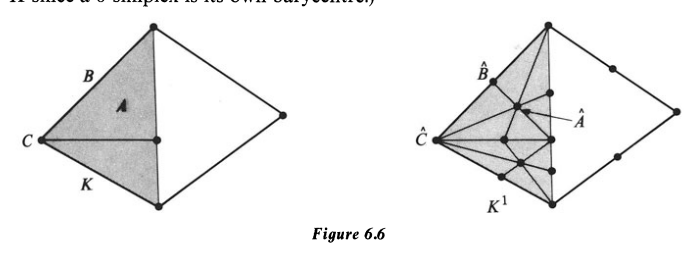
\includegraphics[width=0.8\textwidth]{6.6.png}
    \label{fig:6-6-png}
\end{figure}

\textbf{Lemma 6.4}: The collection of simplexes described above forms
a simplicial complex denoted by $K^{1}$ and called the first barycentric
subdivision of $K$. It has the following properties:\\
(a) each simplex of $K^{1}$ is contained in a simplex of $K$;\\
(b) $\left| K^{1} \right| = \left| K \right| $;\\
(c) if the dimension of $K$ is $n$, then
$\mu (K^{1}) \le \frac{n}{n+1}\mu (K)$.\\
\linebreak

To show (c), we observe that the diameter of a simplex is the length of its
longest edge. Let $\sigma$ be an edge of $K$ with vertices $\hat{A}$ and
$\hat{B}$, say, where $B < A$. Then $\sigma$ is contained in $A$, and if the
dimension of $A$ is $k$ we have
\begin{align*}
\text{length } \sigma
\le \max_i \left\{ 
\|\hat{A} - v_i\|   \right\} 
&= \max_i \left\{ \frac{1}{k+1} \|\sum_{j \neq i} v_j - v_i \|  
\right\} \\
&\le 
\max_i \left\{ \frac{k}{k+1}
\max_j \left\{ \|v_j - v_i\| \right\} \right\} \\
&= \frac{k}{k+1} \max_{i,j} \|v_j - v_i\| \\
&= \frac{k}{k+1} \text{diameter } (A)
\end{align*}
Thus
\[
\text{length }\sigma
\le \frac{k}{k_1} \text{diameter}(A)
\le \frac{n}{n+1} \text{diameter}(A)
\le \frac{n}{n+1} \mu(K)
\] 
Therefore
$\mu (K^{1}) \le \frac{n}{n+1}\mu(K)$.\\
\linebreak


\subsubsection*{Simplicial approximations}
\textbf{Def 6.5:} Let $K$ and $L$ be simplicial complexes. A function
$s  \colon \left| K \right| \to \left| L \right| $ is called simplicial
if it takes simplexes of $K$ linearly onto simplexes of $L$.\\
\linebreak
This means that if $A$ is a simplex of $K$, we require $s(A)$ to be a simplex
of $L$ ; the linearity means that if $A$ has vertices $v_0, v_1, \ldots, v_k$
and
if $x \in A$ is the point $x = \lambda_0 v_0 + \lambda_1 v_1 + \ldots
+ \lambda_k v_k$, where the $\lambda_i$ are nonnegative and
$\sum \lambda_i = 1$, then $s(x)$ when expressed in terms of the vertices of
$s(A)$ is $s(x) = \lambda_0 s(v_0) + \lambda_1 s(v_1)
+ \ldots + \lambda_k s(v_k)$. Note that $s(A)$ may have lower dimension than
$A$ (we do not require $s$ to be injective), in which case
$s(v_0), \ldots, s(v_k)$ will not all be distinct.\\
\linebreak
Simplicial functions are continuous since they are linear functions between
simplexes (and hence continuous) and the gluing lemma ensures continuity on all
of $K$.\\
\linebreak
Because of its linearity on each simplex of $K$, a simplicial map $s$ is
completely determined once we know its effect on the vertices of $K$. In fact,
if a function $s$ from the vertices of $K$ to the vertices of $L$ has the
property that if vertices $v_0, v_1, \ldots, v_k$ determine a simplex of
$K$ then $s(v_0), \ldots, s(v_k)$ determine a simplex of $L$, then
$s$ can be extended linearly across each simplex of $K$ to give a simplicial
map
$\left| K \right| \to \left| L \right| $. In particular, an isomorphism from
$K$ to $L$ extends in this way to a simplicial homeomorphism from the
polyhedron of $K$ to the polyhedron of $L$.\\
\linebreak
\textbf{Def:} Now let $f  \colon \left| K \right| \to \left| L \right| $ be
a map between polyhedra. Given a point
$x \in \left| K \right| $, the point
$f(x)$ lies in the interior of a unique simplex of $L$. Call this simplex the
\textit{carrier} of $f(x)$.\\
\linebreak
\textbf{Def 6.6:} A simplicial map $s  \colon \left| K \right| \to 
\left| L \right| $ is a simplicial approximation of
$f  \colon \left| K \right| \to 
\left| L \right| $ if $s(x)$ lies in the carrier of
$f(x)$ for each $x \in \left| K \right| $.\\
\linebreak
It follows immediately from the definition that $s$ and $f$ are homotopic, for
suppose $L$ lies in $\mathbb{E}^{n}$, and let
$F  \colon \left| K \right| \times I \to \mathbb{E}^{n}$ denote the
straight-line homotopy defined by
$F(x,t) = (1-t) s(x) + t f(x)$. Given $x \in \left| K \right| $, we know that
some simplex of $L$ contains $s(x)$ and $f(x)$ and, since a simplex is convex,
all
points $(1-t)(s) + tf(x)$, $0 \le t\le 1$, must also lie in this simplex.
Therefore the image of $F$ lies in $\left| L \right| $, and $F$ is a homotopy
from $s$ to $f$.\\
\linebreak
\textbf{Simplicial approximations do not always exist; example 6.8:}
Let $\left| K \right|  = \left| L \right|  = \left[ 0,1 \right] $ with
$K$ having vertices at the points 
$0, \frac{1}{3}, 1$ and $L$ at $0, \frac{2}{3}, 1$. Suppose
the given map $f \colon \left| K \right| \to \left| L \right| $ is 
$f(x) = x^2$. Then $f$ does not admit a simplicial approximation.\\
Here, the simplicial complexes do not include $\left[ 0,1 \right] $ as a 
$1$-simplex, since the intersection of this simplex with either
$\left[ 0,\frac{1}{3} \right] $ in $K$ or $\left[ 0, \frac{2}{3} \right] $ in
$L$ is not a face of $\left[ 0,1 \right] $, whose only faces are
$0$ and $1$.\\
Now, with this in mind, we show that there does not exist a simplicial
approximation.\\
Suppose such a simplicial approximation $s  \colon \left| K \right| \to 
\left| L \right| $ exists. Then for any vertex $v$ of $L$,
$s \left( f^{-1}(v) \right) = v$ since $v$ is a $0$-simplex and thus
the carrier of $v$ is $v$ itself. Hence
$s \left( f^{-1}(v) \right) $ must lie in the carrier which is $v$, giving the
equality. So
$s(0) = 0, s(1) = 1$ and $s\left( \sqrt{\frac{2}{3}}  \right) 
= \frac{2}{3}$.\\
Now, $s$ is simplicial, so it must take
$\left[ 0,\frac{1}{3} \right] $ to a simplex in $L$. If
$\left[ 0,\frac{1}{3} \right] $ were mapped to $0$, then
$\left[ \frac{1}{3},1 \right] $ has nothing to be mapped to: it must be mapped
to  $\left[ 0,1 \right] $ to agree with $s(\frac{1}{3}) = 0$ and
$s(1) = 1$, however, then $s$ does not take the simplex
$\left[ \frac{1}{3},1 \right] $ to a simplex in $L$ as $\left[ 0,1 \right] $ is
not a simplex. Similar reasoning shows that 
$\left[ 0,\frac{1}{3} \right] $ cannot be mapped to $\frac{2}{3}$ or $1$.\\
If $\left[ 0,\frac{1}{3} \right] $ were mapped to
$\left[ \frac{2}{3},1 \right] $ then $s(0) = \frac{2}{3}$ by linearity,
contradiction, so $s$ must map it to
$\left[ 0, \frac{2}{3} \right] $ and hence
$s(\frac{1}{3}) = \frac{2}{3}$. However, then
$s(\frac{1}{2}) \in \left[ \frac{2}{3},1 \right] $ which is not the carrier for
$f(\frac{1}{2})$ whose carrier is 
$\left[ 0, \frac{2}{3} \right] $. This shows that $s$ is not simplicial.\\
\linebreak
One can similarly show that there is no simplicial approximation for
$K^{1}$. There is one for $K^{2}$, however.\\
Map $\left[ 0,\frac{1}{2} \right] $ to $0$,
$\left[ \frac{1}{2},\frac{2}{3} \right] $ to $\left[ 0, \frac{2}{3} \right]
$ linearly, $\left[ \frac{2}{3},\frac{5}{6} \right] $ to
$\frac{2}{3}$ and $\left[ \frac{5}{6},1 \right] $ to
$\left[ \frac{2}{3},1 \right] $ linearly.\\
\linebreak
Firstly, this map satisfies that
$s(0) = 0, s(1)=1$ and $s\left( \sqrt{\frac{2}{3}}  \right) 
= \frac{2}{3}$.\\
Now, the below figure shows that the mapping is indeed simplicial.
\begin{figure}[H]
    \centering
    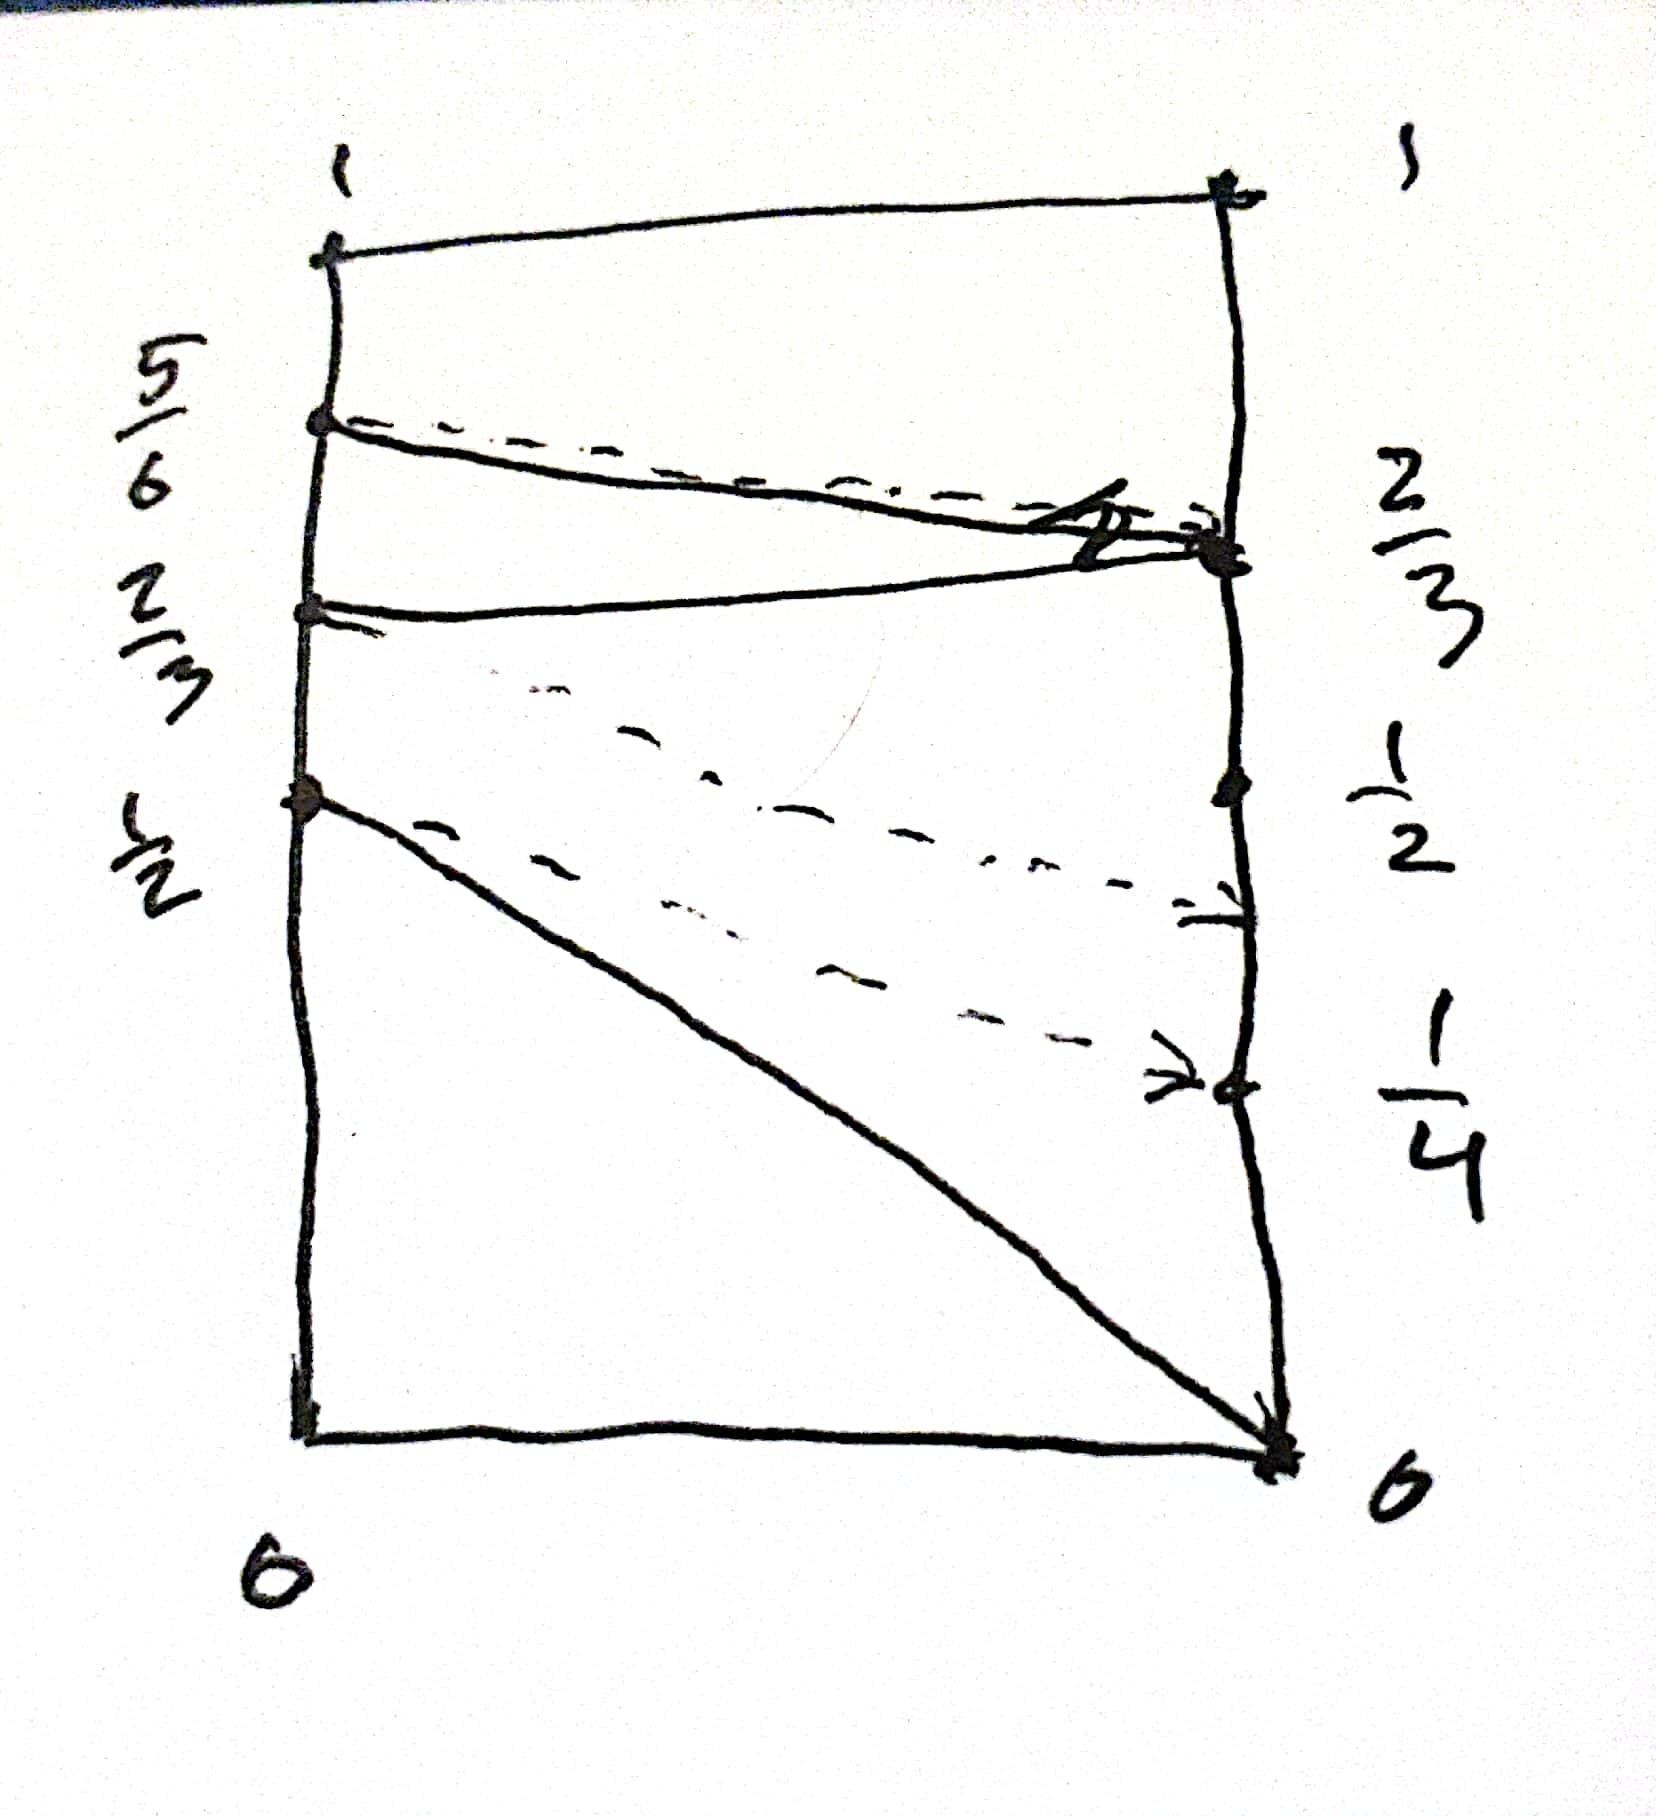
\includegraphics[width=0.4\textwidth]{ex6.8.jpeg}
    \label{fig:ex6-8-jpeg}
\end{figure}
So why is it impossible for $K^{1}$? Well, there we have that
$\sqrt{\frac{2}{3}} $ lies in
$\left[ \frac{2}{3},1 \right] $ in $K$, 
and since $s \left( \sqrt{\frac{2}{3}}  \right) = \frac{2}{3}$ and
$s (1) = 1$ and $s$ maps $\left[ \frac{2}{3},1 \right] $ to a simplex, it maps
$\left[ \frac{2}{3},1 \right] $ to a simplex containing both $1$ and
$\frac{2}{3}$. The only such simplex is $\left[ \frac{2}{3},1 \right] $, so
$s$ maps $\left[ \frac{2}{3},1 \right] $ to
$\left[ \frac{2}{3},1 \right] $. Now, $s$ maps this linearly, so we have that
$\frac{2}{3} = s\left( \sqrt{\frac{2}{3}}  \right) 
= s\left( \lambda_0 \cdot \frac{2}{3} + (1- \lambda_0) \cdot 1 \right) 
= \lambda_0 \cdot \frac{2}{3} + 1 - \lambda_0
= 1 - \frac{\lambda_0}{3}$. So $\lambda_0 = 1$, however
 
$\sqrt{\frac{2}{3}}\neq 
\frac{2}{3}$, contradiction.\\
\linebreak
\textbf{Def:} Let $K$ be a complex and let $v$ be a vertex of $K$. The
\textit{open star} of $v$ in $K$ is the union of the interiors of those
simplexes of $K$ which have $v$ as a vertex. It is an open subset of $\left| K \right| $ 
and we denote it by $\text{star}(v, K)$.
\begin{figure}[H]
    \centering
    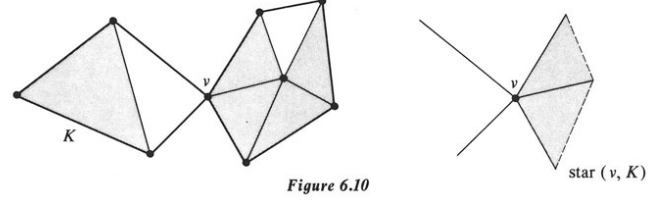
\includegraphics[width=0.6\textwidth]{star.png}
    \label{fig:star-png}
\end{figure}

\textbf{Lemma 6.9:} Vertices $v_0, v_1, \ldots, v_k$ of a simplicial complex
$K$ span (i.e. are the vertices of) a simplex of $K$ if and only if the
intersection of their open stars is nonempty.\\
\linebreak
\textbf{Proof:} If $v_0, \ldots, v_k$ are the vertices of the simplex $A$ of
$K$ then the whole of the interior of $A$ lies in $\text{star}(v_i, K)$ for
$0 \le  i \le k$. Conversely, suppose that 
$x \in \bigcap_{0}^{k}\text{star}(v_i, K)$ and let $A$ be the carrier of $x$.
By the definition of an open star, each $v_i$ must be a vertex of
$A$, and therefore $v_0, \ldots, v_k$ span some face of $A$.\\
\linebreak
We use this for the following theorem:\\
\textbf{Theorem 6.7: Simplicial approximation theorem:} Let $f \colon \left| K \right| 
\to \left| L \right| $ be a map between polyhedra. If
$m$ is chosen large enough there is a simplicial approximation
$s  \colon \left| K^{m} \right| 
\to \left| L \right| $ to
$f  \colon \left| K^{m} \right| \to L$.\\
\linebreak
\textbf{Proof:} We first deal with the special case of the theorem where
it is not necessary to chop up/refine the simplexes of $K$.\\
Suppose that for each vertex $u$ of $K$, we can ind a vertex
$v$ of $L$ satisfying the inclusion
\[
f\left( \text{star}(u, K) \right) 
\subset \text{star}(v,L) \tag{$\Omega$}
\] 
Define a function $s$ from the vertices of $K$ to those of $L$ by choosing such
a $v$ for each $u$ and setting $s(u) = v$. Then suppose that
$u_0, \ldots, u_k$ span a simplex of $K$. \\
By construction,
\[
\bigcap_{0}^{k} \text{star}(s(u_i),L)
\supset \bigcap_{0}^{k} f\left( \text{star}(u_i,K) \right) 
= f \left( \underbrace{\bigcap_{0}^{k}\text{star}(u_i,K)}_{\neq \varnothing} \right) 
\tag{$\alpha$}
\] 
where we have $\neq \varnothing$ by lemma 6.9. and the inclusion
from $\Omega$.\\
Now we can therefore extend $s$ linearly over each simplex of $K$ to give a 
simplicial map $s  \colon \left| K \right| \to 
\left| L \right| $. This map
$s$ simplicially approximates $f$: for let
$x \in \left| K \right| $ and let $u_0, \ldots, u_k$ be the vertices of
its carrier. Then $x \in \bigcap \text{star}(u_i,K)$, so by
the $\alpha$, we have
$f(x) \in \bigcap \text{star}(s(u_i),L) $, so
the carrier of $f(x)$ in $L$ has the simplex spanned by
$s(u_0), \ldots, s(u_k)$ as a face, and consequently, it must contain the
point $s(x)$ which lies in this face.\\
\linebreak
To deal with the theorem in general, we need only show that we can arrange
for the inclusion ($\Omega$) to be satisfied at the expense of replacing
$K$ by a suitable barycentric subdivision $K^{m}$.\\
\linebreak
\textbf{6.3.(13):} Use the simplicial approximation theorem to show that the
$n$-sphere is simply connected for $n\ge 2$.\\
\linebreak
\textit{Solution:}
Suppose $\gamma  \colon I \to S^{n}$ is a path.\\
Since $S^{n}$ is homeomorphic to an $n+1$-simplex which is a polyhedra and
$I$ is a $1$-simplex and a polyhedra, we have by the simplicial approximation
theorem that there exists some $m \in \mathbb{N}$ such that
$s  \colon \left| I^{m} \right| \to \left| \Delta^{n+1} \right| $ is a simplicial
approximation to $f  \colon \left| I^{m} \right| \to  \left| \Delta^{n+1}
\right|$. Then $s$ and $f$ are homotopic. Furthermore, we can assume that
$\gamma$ starts at a vertex of the $n+1$-simplex. Now, $s$ takes simplexes to
simplexes, so letting $v_0, \ldots, v_k$ be the vertices of $I^{m}$,
$s\left( \left[ v_i, v_{i+1} \right]  \right) $ is a simplex of
the $n+1$-simplex. Linearity of $s$ implies that the simplex is of dimension
$0$ or $1$, i.e. $s$ lives completely on $1$-simplex faces of the
$n+1$-simplex. Thus  $s$ is not onto, so
$\gamma$ is nullhomotopic.\\
\linebreak
\textbf{14:} If $k < m,n$, show that any map from
$S^{k}$ to $S^{m}$ is null homotopic, and that the same is true of any map from
$S^{k}$ to $S^{m} \times S^{n}$.\\
\linebreak
\textit{Solution:} 
Suppose $f  \colon S^{k} \to S^{m}$ is a map for $k<m$. 
Let $g  \colon \left| K \right| \to 
S^{k}$ be a triangulation of $S^{k}$ and
$h  \colon \left| L \right| \to 
S^{m}$ a triangulation of $S^{m}$ to an $k+1$ and $m+1$ simplex, resp. Then
$h^{-1} \circ f \circ g$ is a map of complexes which has a simplicial
approximation
$s  \colon \left| K^{m} \right| 
\to \left| L \right| $.
But $\dim \left| K^{m} \right| = \dim \left| K \right| 
< \dim \left| L \right| $, so as $s$ maps simplexes to simplexes of lesser or
equal dimension, the dimension of the image of $s$ is of degree at most
$k+1 < m+1$, so $s$ is not surjective. For a point
$p \not\in s \left( \left| K^{m} \right|  \right) $, we have that
$\left| L \right| - \left\{ p \right\} 
\cong S^{m} - \left\{ h(p) \right\} 
\cong \mathbb{R}^{m}$, so
$s$ is nulhomotopic as $\mathbb{R}^{m}$ is convex.\\
Now $s \simeq h^{-1} \circ f \circ g \simeq f$, so
$f$ is nulhomotopic.

\subsection*{Triangulating orbit spaces}
Let $K \subset \mathbb{E}^{n}$ be a simplicial complex whose simplexes lie in
$\mathbb{E}^{n}$. Let $V$ denote the set of vertices of $K$ and
$S$ the collection of those subsets of $V$ which span simplexes of $K$.\\
The pair $\left\{ V, S \right\} $ is called the \textbf{vertex scheme} of 
$K$. The set $V$ is finite and $S$ has the following properties:
\begin{enumerate}
    \item Each element of $V$ belongs to $S$ (A vertex is a $0$-simplex)
    \item If $X$ belongs to $S$ then any nonempty subset of $X$ belongs to 
        $S$ (Any face of a simplex of $K$ is itself in $K$ )
    \item The sets in $S$ are nonempty and have at most $m+1$ elements for some
        non-negative integer $m$.
\end{enumerate}
\textbf{Def.} \textbf{Realization} means finding a simplicial complex $K$, and
a bijection from $V$ to the set of vertices of $K$, so that memebers of $S$
correspond exactly to those sets of vertices which span simplexes.\\
\linebreak
\textbf{6.14. Realization theorem.} Let $V$ be a finite nonempty set
and $S$ a collection of subsets of $V$ which satisfies properties
(a)-(c) listed above. Then $\left\{ V,S \right\} $ can be realized as the
vertex scheme of a simplicial complex.\\
\linebreak



\subsection*{Simplicial homology}
\textbf{Problem 8.2.2:} Show that the elementary 1-cyles generates
$Z_1(K)$ for any complex $K$.\\
\linebreak
\textit{Solution:} Suppose
$\lambda_1 (u_1, v_1) + \ldots + \lambda_k (u_k, v_k)$ is an arbitrary element
of $Z_1(K)$. Then define
$G = \left\{ 
(u,v)  \mid u,v \text{ are 0-simplexes of }K \right\} $.
Then $\lambda_1 (u_1, v_1)
+ \ldots + \lambda_k (u_k, v_k) \in 
\langle G \rangle $ and clearly
$\langle G \rangle \subset 
\left\{ 
\lambda_1 (u_1, v_1) + \ldots + 
\lambda_k (u_k, v_k)  \mid 
\lambda_i \in \mathbb{Z}, u_i,v_j \text{ are 0-simplexes of }K \right\} $.





\textbf{Lemma 8.8:} $\chi$ is a chain map.\\
\linebreak
\textit{Solution:} Suppose $\sigma = \left( v_0, \ldots, v_k, v_{k+1}, \ldots
,v_q \right) $ and $v_0, \ldots, v_k$ are the vertices of $A$. Then
\[
\chi \left( \sigma \right) 
= \sum_{i=0}^{k} (-1)^{i} \left( v, v_0, \ldots,
 \hat{v_i}, \ldots, v_k, v_{k+1}, \ldots, v_q \right).
\] 
If $\sigma$ does not have $A$ as a face we set 
$\chi (\sigma) = \sigma$.\\
Now
\begin{align*}
    \partial \chi (\sigma)
    &= \partial \sum_{i=0}^{k} (-1)^{i}
    \left( v, v_0, \ldots, \hat{v_i}, \ldots, v_k, v_{k+1}, \ldots, v_q
    \right)\\
    &= \sum_{i=0}^{k} (-1)^{i} \left( v_0, \ldots, \hat{v_i},\ldots,
    v_k, \ldots, v_q\right) 
    + \sum_{i=0}^{k} \sum_{j=0}^{i-1} (-1)^{i +j +1} \left( v,
    \ldots, \hat{v_j}, \ldots, \hat{v_i}, \ldots, v_k, \ldots, v_q\right)\\
    &+ \sum_{i=0}^{k} \sum_{j=i+1}^{q} (-1)^{i+j}
    (v, \ldots, \hat{v_i}, \ldots, \hat{v_j}, \ldots, v_k,\ldots, v_q)\\
\end{align*}
And
\begin{align*}
\chi \partial \sigma
&= \chi \sum_{i=0}^{q} (-1)^{i} \left( 
v_0, \ldots, \hat{v_i}, \ldots, v_q \right)\\
&= \sum_{j=0}^{k} (-1)^{i} \left( 
v_0 ,\ldots, \hat{v_i} , \ldots, v_{k+1}, \ldots, v_q \right)
+ \sum_{i=k+1}^{q} \sum_{j=0}^{k} (-1)^{i+j}
\left( v, v_0, \ldots, \hat{v_j},\ldots, v_k, \ldots, \hat{v_i},\ldots, v_q \right) 
\end{align*}






\end{document}
